\documentclass{scrreprt}
\usepackage[margin=0.7in]{geometry} %réduire marges

\setkomafont{disposition}{\normalfont\bfseries}

%french
\usepackage[utf8]{inputenc}
\usepackage[colorlinks=true,urlcolor=blue,linkcolor=blue]{hyperref}
\usepackage[T1]{fontenc}
\usepackage[francais]{babel} %en Français
\usepackage[pdftex]{graphicx}
\usepackage{listings}
\usepackage{graphicx} %pour les images

\usepackage{xcolor}

\definecolor{Zgris}{rgb}{0.87,0.85,0.85}

\newsavebox{\BBbox}
\newenvironment{DDbox}[1]{
\begin{lrbox}{\BBbox}\begin{minipage}{\linewidth}}
{\end{minipage}\end{lrbox}\noindent\colorbox{Zgris}{\usebox{\BBbox}} \\
[.5cm]}


\begin{document}
\title{Projet PERI}
\subtitle{\textit{Rapport}}
\date{26 mai 2015}
\author{Maxime \textsc{Bittan}, Daniel \textsc{Bourdrez}, Redha \textsc{Gouicem},\\ Alexandra \textsc{Hospital}, Ilyas \textsc{Toumlilt}}


\maketitle

\pagebreak
\tableofcontents

\pagenumbering{arabic}

Dans ce (pas très) court tutoriel, nous allons vous montrer comment 
fabriquer votre propre station météo. Et comme ça serait un peu trop banal, 
votre station météo sera en plus mobile ! Nous proposons pour cela une
architecture assez simple, avec d'un côté une Raspberry Pi qui fera office de
serveur et de gestionnaire, et d'un autre côté une Arduino motorisée faisant
office de station météo.

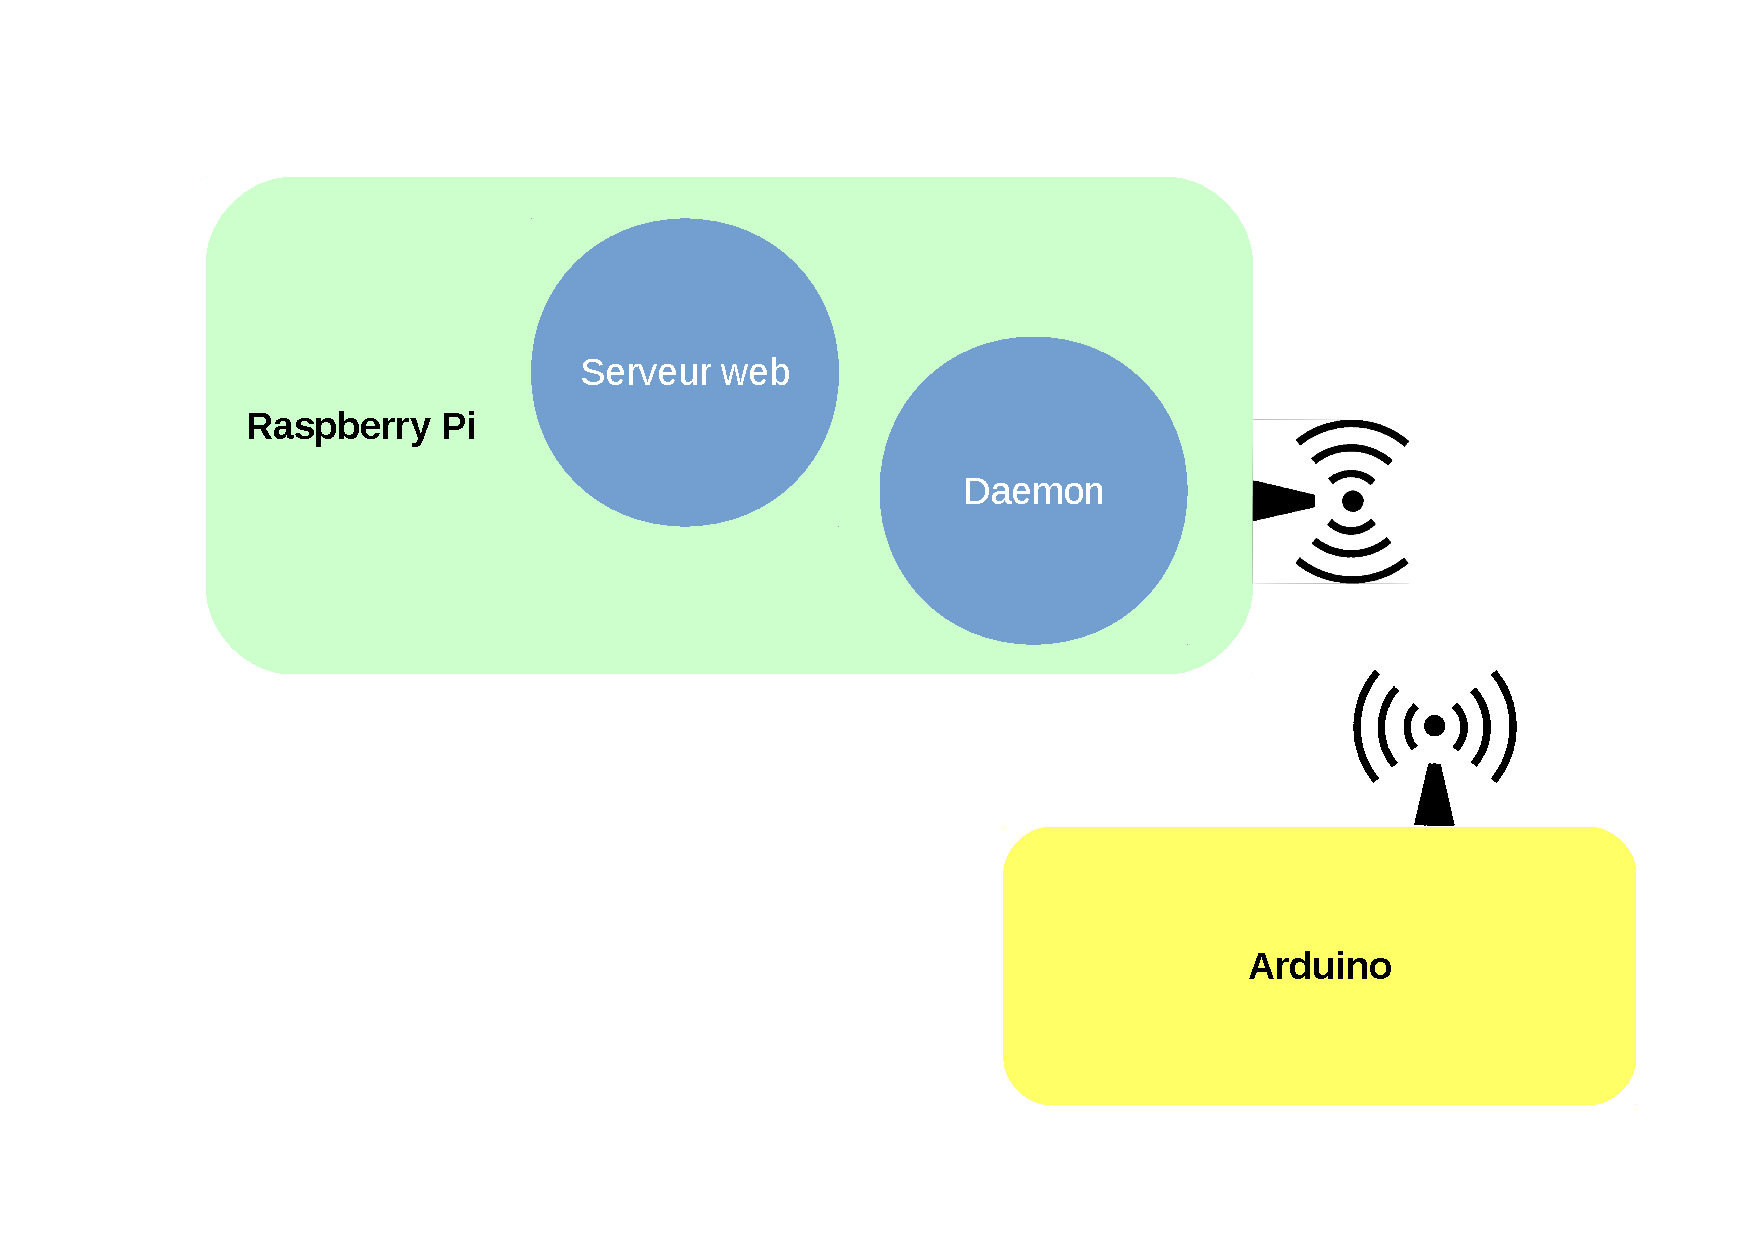
\includegraphics[width=\textwidth]{include/archi.pdf}

On notera que la Raspberry contient deux entités : le serveur web, qui permettra
de tout gérer de l'extérieur, et le daemon, qui fera le lien entre le serveur 
web et l'Arduino par le biais de communications radios.


\chapter{Montage matériel}
Afin de réaliser notre station météo mobile, nous avons deux montages à
réaliser :
\begin{itemize}
\item le serveur (Raspberry Pi)
\item la station mobile (Arduino motorisée)
\end{itemize}

\section{Serveur}

\section{Station mobile}
Le montage sera le suivant :
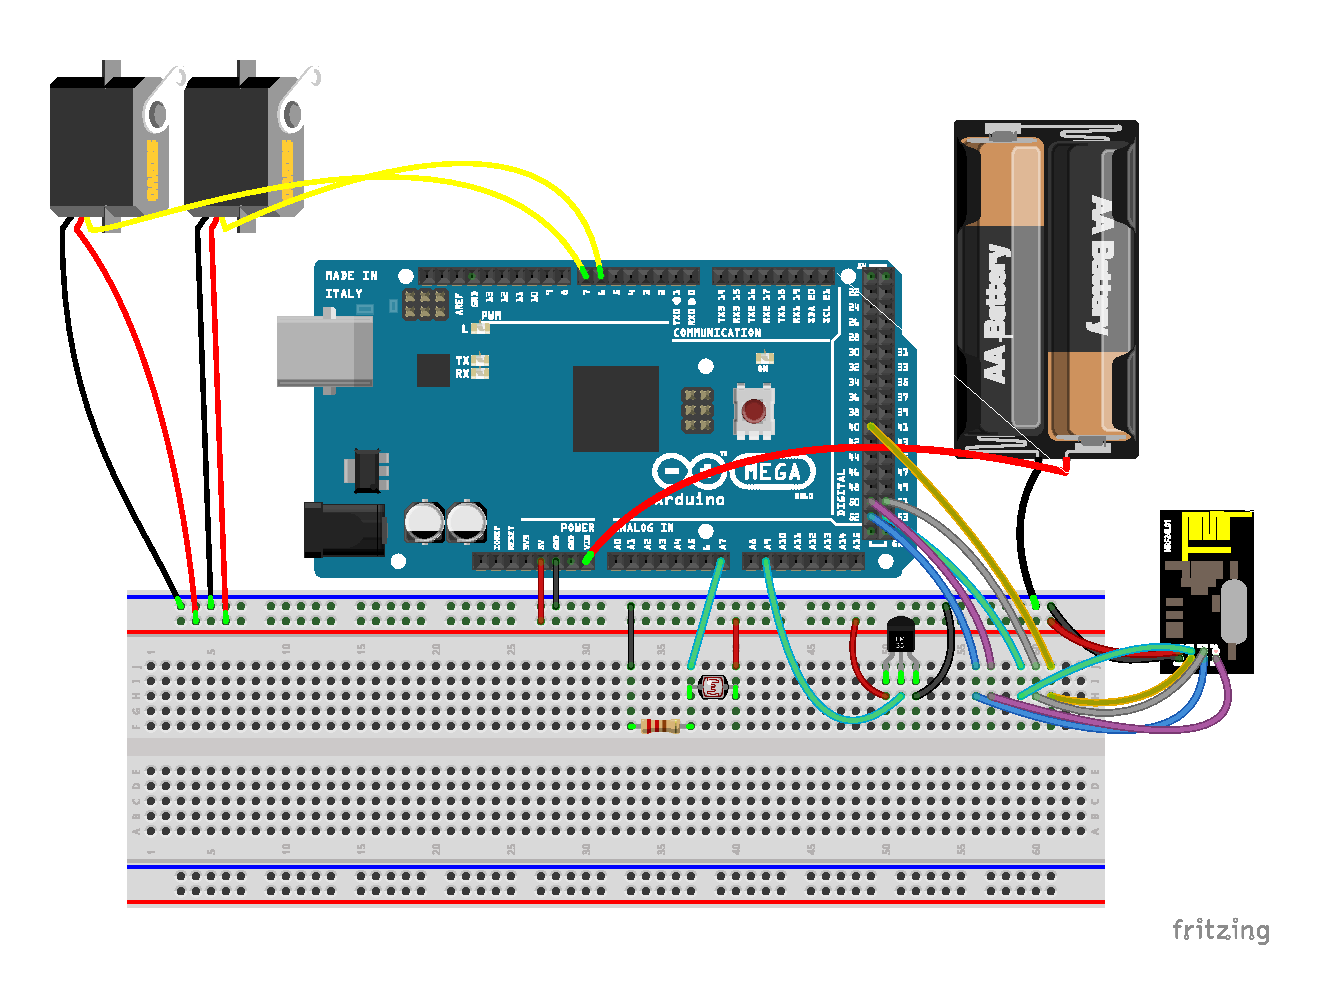
\includegraphics[scale=0.5]{include/arduino_bb.pdf}
\paragraph{}
On ne parlera pas ici de l'aspect mécanique (chassis, placement des moteurs,
etc...).


\chapter{Serveur}
Exécuté sur la Raspberry Pi, sollicité par un ( ou plusieurs ) client(s) d’un côté et un ( ou plusieurs ) démon(s) de l’autre. Le serveur web est la pièce maîtresse de ce projet, il doit pouvoir servir toutes les requêtes, en continu, tout en assurant la cohérence des données transitantes, leur fiabilité, ainsi qu’une gestion intelligente de la mémoire ( les requêtes pouvant facilement atteindre un nombre très considérable ). Nous reviendrons plus en détails sur la nature de ces requêtes ainsi que les implémentations choisies.

\section{Choix de l'environement}

\subsection{Le serveur HTTP}

Entre de simples scripts sh/python en CGI, un NodeJS plus flexible mais peu fiable, nous avons décidé de jouer la carte de la performance - et de l’enchevêtrement aussi, je l’assume - et nous choisîmes donc l’\textbf{Apache2}.\\
Ce serveur HTTP, l’un des plus populaires du World Wide Web, est spécialement adapté pour les environnements UNIX, une harmonie dont nous profiterons pleinement, vu que notre Raspberry Pi tourne sous Linux. Apache2 est également conçu pour prendre en charge de nombreux modules lui donnant des fonctionnalités supplémentaires, nous en utiliserons les suivantes :
\begin{itemize}
\item Interprétation du langage PHP.
\item Serveur Proxy, nécessaire pour l’exécution sur l’environnement de la fac ( ARI alias PPTI ).
\item Common gateway interface.
\item Server sides includes.
\item La réécriture d’URLs.
\item Et quelques protocoles de communication additionnels.
\end{itemize}
( Nous reviendrons sur l’utilisation de ces fonctionnalités quand nous commencerons à voir leur implémentation )

\subsection{Choix des langages}

L’adoption d’Apache2 nous permet donc un choix très large au niveau des langages, cependant, PHP reste le langage le mieux interprété par ce serveur HTTP.\\
PHP est un langage de script, utilisé le plus souvent côté serveur. Dans notre architecture, le serveur Apache2 interprète le code PHP des pages Web ou des scripts demandés et génère du code (HTML, XHTML, CSS par exemple) et des données (JPEG, GIF, PNG par exemple) pouvant être interprétées et rendues par un navigateur web.\\
Autre sa souplesse, PHP nous permettra une gestion assez ``bas niveau'' ( par rapport à ses concurrents, dans le domaine ) de notre serveur Web et de ses protocoles, il implémente également toute la bibliothèque POSIX dont nous allons nous servir pour relayer les données au démon.\\
Un dernier avantage de PHP, et sûrement le plus pertinent, et son côté ``dynamique'' ( ce qui fait majoritairement son succès et son adoption par des géants comme Google, Facebook … ). Une page web dynamique ( par opposition à une page web statique ), et une page dont le contenu peut varier en fonction des informations qui ne sont connues qu’au moment de sa consultation, mieux le contenu de ces pages peut même varier après le chargement et au cours du temps, sans avoir à recharger la page, pour cela nous aurons besoin de définir une méthode de dialogue, entre le navigateur client, et le serveur.\\
\\
Avant de définir cette méthode, nous avons besoin de définir les langages côté client, pour ce côté, on restera dans le classique, HTML + CSS pour l’affichage de la page, et de JavaScript ( JS, JQuery et DOM ) pour les scripts client.
\\
La méthode de dialogue entre le client et le serveur sera donc AJAX, qui permet de construire des sites web dynamique et interactifs, dans notre cas cette communication se fera essentiellement en manipulant des XMLHttpRequest, ainsi :
\begin{itemize}
\item DOM et JavaScript permettent de modifier l'information présentée dans le navigateur en respectant sa structure
\item l'objet XMLHttpRequest sert au dialogue asynchrone avec le serveur Web
\item XML structure les informations transmises entre serveur Web et navigateur.
\end{itemize}

\subsection{Installation de l'environnement}

Afin que tout cela fonctionne, il est nécessaire d’installer quelques outils, le script ./web/install\_env.sh contient les commandes bash nécessaires :\\

\begin{DDbox}{\linewidth}
\begin{lstlisting}[language=bash]
        sudo aptitude update
        sudo aptitude upgrade
        sudo aptitude install apache2
        sudo aptitude install php5
        sudo aptitude install mysql-server php5-mysql
        sudo rm /var/www/index.html
        echo "<?php phpinfo(); ?>" > /var/www/index.php
\end{lstlisting}
\end{DDbox}
\\
Vous l’aurez donc compris, les sources php doivent se trouver dans /var/www/ pour être interprétées, chemin dont le point d’entrée est http://localhost/ , depuis un navigateur web.


\section{Conception du serveur Web}

De manière plus conceptuelle, le client a besoin de pouvoir générer la page web depuis son navigateur ( nous reviendrons sur les composants de cette page ) et donc y avoir un accès par URL, cette adresse devrait mener, du point de vue de notre projet, au point d’entrée du serveur, c’est à dire dans le cas d’un serveur php, le fichier index.php placé à la racine du projet.\\
Le client aura ensuite besoin de transmettre des commandes asynchrones et dynamiques pour modifier les données sur son interface ou pour donner des ordres ( commandes ) au serveur, pour cela nous utiliserons le protocole AJAX décrit plus haut.\\
Finalement, et d’un autre côté, le démon utilisera, pour ses communications avec le serveur des pipes fifo Posix.

\section{Retour sur la station météo mobile}

Maintenant que l’environnement, langages et protocoles ont été définis, nous pouvons y refléter le but de notre projet, en effet, contrôler la voiture signifie envoyer des commandes vers celle-ci, le client devrait donc pouvoir, à l’aide de la page web générée, envoyer des commandes asynchrones, contrôlant la vitesse ou l’orientation, cette commande, et comme présenté plus haut, sera relayée grâce à l’AJAX qui va réveiller un script cible sur le serveur destiné à traiter cette commande, dans notre cas, l’écriture d’une commande correspond à son transfert sur le pipe du démon. Une autre partie du projet consiste à recueillir les informations relatives à la température et luminosité pour les afficher sur la page web, pour cela les scripts serveur devront lire sur le pipe démon qui fournira ces données, et les écrire sur les champs dédiés de l’interface, en passant encore par le moyen de communication asynchrone, AJAX.

\section{La page web principale - IHM}

Générée à la demande par l’utilisateur depuis un URL, elle se compose d’une interface web ( HTML + CSS ), et d’un ensemble de scipts JavaScript permettant le dynamisme et implémentant en utilisant JQuery et DOM, l’IHM ( Interface Homme-Machine ).

\subsection{Les bibliothèques utilisées}

Tant utiles pour l’ergonomie que pour leur facilité d’utilisation, les bibliothèques graphiques ( ou CssLibs pour les HTMLiens ) nous offrent des avantages très considérables dont nous allons profiter, le but est simple : avoir une interface simple, jolie et réactive, sans coder une seule ligne pour l’implémenter.\\
Ces librairies se trouvent dans ./web/lib/\\
\\
\textbf{Twitter Boostrap :}\\
Très connu pour la création de sites et d’applications web, bootstrap est une collection d’outils contenant des codes HTML et CSS, des formulaires, boutons et autres éléments interactifs, ainsi que des extension JavaScript en option.
\\
\textbf{Extended Bootstrap:}\\
Une version étendue de Bootstrap, que j’ai développé moi-même l’été dernier et qui contient un ensemble de scripts ( js ) permettant d’avoir des pages web en responsive design, version mobile mais surtout surcouchant la classe plot, permettant de dessiner des graphes et schéma, dont on va nous servir pour éviter de passer par google charts.\\
Une documentation en version html de cette lib est disponible dans ./web/lib/doc/\\
\\
\textbf{Jquery :}\\
Une biblithèque javascript permettant de parcourir et modifier le DOM ( arbre syntaxique de la page HTML ) et la gestion des événements et de effets visuels.\\
\\
On va donc commencer par inclure toutes ses libs dans notre page HTML :\\
\\
Les CSS dans les headers :\\
\begin{DDbox}{\linewidth}
\begin{lstlisting}[language=html]
  <link rel='stylesheet' media='all' type='text/css' href='./lib/bootstrap-3.3.4/dist/css/bootstrap.css' />
	 <!-- extended bootstrapCss -->
	 <link href="lib/extendedBootstrap/css/bootstrap.min.css" rel="stylesheet" />
	 <link href="lib/extendedBootstrap/css/font-awesome.min.css" rel="stylesheet" />

	 <link rel="stylesheet" href="lib/extendedBootstrap/css/jquery-ui-1.10.3.custom.min.css" />
	 <link rel="stylesheet" href="lib/extendedBootstrap/css/chosen.css" />
	 <link rel="stylesheet" href="lib/extendedBootstrap/css/datepicker.css" />
	 <link rel="stylesheet" href="lib/extendedBootstrap/css/bootstrap-timepicker.css" />
	 <link rel="stylesheet" href="lib/extendedBootstrap/css/colorpicker.css" />
	 <link href="lib/extendedBootstrap/css/refineslide.css" rel="stylesheet" />
	 <link href="lib/extendedBootstrap/css/bootstro.css" rel="stylesheet" />

	 <link rel="stylesheet" href="lib/extendedBootstrap/css/jquery-slider.css" />
	 <link rel="stylesheet" href="lib/extendedBootstrap/css/checkbox-radio-switch.css" />
	 <link href="lib/extendedBootstrap/css/extend.css" rel="stylesheet" />
\end{lstlisting}
\end{DDbox}
\\
Et les JS à la fin du body juste avant de fermer </body> :\\
\begin{DDbox}{\linewidth}
\begin{lstlisting}[language=html]
  <script src="lib/extendedBootstrap/js/bootstrap.min.js"></script>
      <script src="lib/extendedBootstrap/js/jquery-ui-1.10.3.custom.min.js"></script>

      <script src="lib/extendedBootstrap/js/flot/jquery.flot.min.js"></script>
      <script src="lib/extendedBootstrap/js/flot/jquery.flot.pie.min.js"></script>
      <script src="lib/extendedBootstrap/js/flot/jquery.flot.resize.min.js"></script>

      <script src="lib/extendedBootstrap/js/date-time/bootstrap-datepicker.min.js"></script>
      <script src="lib/extendedBootstrap/js/date-time/bootstrap-timepicker.min.js"></script>
      <script src="lib/extendedBootstrap/js/bootstrap-colorpicker.min.js"></script>

      <script src="lib/extendedBootstrap/js/jquery.knob.min.js"></script>
      <script src="lib/extendedBootstrap/js/jquery.autosize-min.js"></script>
      <script src="lib/extendedBootstrap/js/jquery.inputlimiter.1.3.1.min.js"></script>
      <script src="lib/extendedBootstrap/js/jquery.maskedinput.min.js"></script>
      <script src="lib/extendedBootstrap/js/jquery.refineslide.js"></script>
      <script src="lib/extendedBootstrap/js/bootbox.js"></script>
      <script src="lib/extendedBootstrap/js/bootstro.min.js"></script>
\end{lstlisting}
\end{DDbox}

\subsection{Architecture de la page principale}

La page principale se compose de trois champs majeurs :
\begin{itemize}
\item Control de la voiture
\item Temperature
\item Luminosité
\end{itemize}

Ces champs sont des balises div, dont l’attribut id identifie de manière unique chacun des 3 :\\
\begin{DDbox}{\linewidth}
\begin{lstlisting}[language=html]
  <div id='carControlContainer' >

  </div>
  
  <div id='temperatureContainer' >

  </div>

  <div id='graphContainer' >

  </div>
\end{lstlisting}
\end{DDbox}
\\
Le corps de chaque composant sera représenté par un panel Bootstrap, dont la structure est la suivante :\\
\begin{DDbox}{\linewidth}
\begin{lstlisting}[language=html]
  <div class="panel panel-default">
	    <div class="panel-heading">
	       <h3 class="panel-title">
		  ICI LE TITRE DU PANEL
	       </h3>
	    </div>
	    <div class="panel-body">
	       ICI LE CORPS DU PANEL
	    </div>
	 </div>
\end{lstlisting}
\end{DDbox}
\\
Bootstrap et ExtendedBoostrap s'occupent de gérer la mise en forme et la mise en page selon la taille de la fenêtre, il suffit par exemple ici de leur indiquer l'attribut class d'une balise pour qu'ils sachent ce qu'il faut faire.
\\
\\
A partir de là, à chaque fois que nous parlerons du contenu d'une section, on fera directement référence au corps du panel.

\subsection{Car control}

Dans cette partie, nous avons besoin d'interactions à double-sens, c’est à dire, et avoir des objets cliquables pour envoyer nos commandes, et pouvoir afficher l’été actuel de ces valeurs, on a donc opté pour des barres deux barres de défilement, une pour contrôler la vitesse de la voiture et une autre pour contrôler son orientation, les deux barres son munies de deux flèches pour chaque extrémité permettant d’incrémenter/décrémenter les valeurs.\\
Le changement des valeurs et la gestion du clique seront traitées ultérieurement.

\subsection{Weather station}

Cette partie ne fait qu'afficher en texte brut la valeur de la température.

\subsection{Brightness graph}

La partie la plus compliquée graphiquement, elle contient le graphe qui devrait afficher en temps-réel les valeurs de luminosité reçues. Ce graphe est représenté par un canvas où on commence par dessiner les deux axes et les légendes, puis une fois l’ensemble créé, un fichier js intervient, il s’agit de :\\
\begin{DDbox}{\linewidth}
\begin{lstlisting}[language=html]
<script src='./js/charts-flot.js'></script>
\end{lstlisting}
\end{DDbox}
\\
Ce fichier définit quelques fonctions essentielles à la gestion du graphe, la partie qui nous intéresse ici est contenue dans
\begin{lstlisting}[language=java]
  $(document).ready{}
  \end{lstlisting}
et qui veut dire ``exécute mon corps au chargement de la page'', cette partie contient un tableau de donnée data, qu’on initialise de la sorte :\\
\begin{DDbox}{\linewidth}
  \begin{lstlisting}[language=java]
  function initChart() {
      for(var i = 0; i < totalPoints; i++){
	 data.push(0);
	 res.push([i, 0]);
      }
      
      return res;
   }
\end{lstlisting}
\end{DDbox}
\\
( res étant une hashmap associant à chaque point de l’axe des y, une valeur data correspondante )
Nous passons ensuite à l’initialisaion du plot :\\
\begin{DDbox}{\linewidth}
\begin{lstlisting}[language=java]
  var plot = $.plot($("#realtimechart"), [initChart()], options);
\end{lstlisting}
\end{DDbox}
\\
et à un premier dessin :\\
\begin{DDbox}{\linewidth}
\begin{lstlisting}[language=java]
  plot.setData([res]);
plot.draw();
\end{lstlisting}
\end{DDbox}
\\
La suite est donc intuitive, à chaque réception de donnée, on la rajoute au tableau data et on update le chart :\\
\begin{DDbox}{\linewidth}
\begin{lstlisting}[language=java]
  function updateChart(newValue) {
      if( data.length > 0)
	 data = data.slice(1);
      
      data.push(newValue);
      
      // zip the generated y values with the x values
      res = [];
      for(var i = 0; i < data.length; i++){
	 res.push([i, data[i]]);
      }
      
   }
\end{lstlisting}
\end{DDbox}

\section{L'interface AJAX}

Gère les communication entre le client et le serveur, composée de fichier javascripts côté client et de scripts PHP côté serveur, nous allons commencer par inclure nos fichiers js sur la page principale :\\
\begin{DDbox}{\linewidth}
\begin{lstlisting}[language=html]
  <script src='./ajax/ajax.js'></script>
	 <script src='./js/charts-flot.js'></script>
	 <script src='./js/speedUp.js'></script>
	 <script src='./js/turn.js'></script>
	 <script src='./js/temperature.js'></script>
\end{lstlisting}
\end{DDbox}
\\
Le premier ( ajax.js ) implémente les fonctions permettant d'envoyer nos requêtes HTTP vers le serveur, on utilise une instance la classe XMLHTTPRequest(), à la quelle on associe l'URL cible et la fonction js cible à appeler en cas de réponse, ansi que les données à envoyer sous forme de paramètres en POST. Le corps de la fonction est simple, et nous donne :\\
\begin{DDbox}{\linewidth}
\begin{lstlisting}[language=java]
  function ajax_brightness(url, flux, rappel, arg, method) {
  var r = window.XMLHttpRequest ? new XMLHttpRequest() :
    (window.ActiveXObject ?  new ActiveXObject("Microsoft.XMLHTTP") : '');
  if (!r) return false;
  r.onreadystatechange = function () {rappel(r, arg);};
  r.open(method ? method : 'POST', url, true);
  if (flux)
      r.setRequestHeader("Content-Type", 
                         "application/x-www-form-urlencoded; ");
  r.send(flux);
  return true;
}
\end{lstlisting}
\end{DDbox}
\\
Les autres fichiers contiennent justement ces fonctions de rappel, en plus des fonctions de déclenchement ( par timeout ou par clique selon le besoin ) des requêtes AJAX.\\
Prenons pour exemple la temperature, le fichier temperature.js se charge de gérer le champ température, chaque seconde il fait appel à :\\
\begin{DDbox}{\linewidth}
\begin{lstlisting}[language=java]
var temperatureUpdateInterval = 1000;
   function updateTemperature() {
      if( !tempLock ){
	 tempLock = 1;
	 document.getElementById("temperatureLoading").style.display = "initial";
	 ajax_temperature("./ajax/temperatureAjax.php", 0, receiveTemperature, 0);
      }
      setTimeout(updateTemperature, temperatureUpdateInterval);
   }
\end{lstlisting}
\end{DDbox}
\\
cette fonction s'occupe d'appeler, en passant par le script ajax, le script PHP serveur temperatureAjax.php, qui se charge lire dans le pipe et renvoyer en texte brut la valeur de la temperature ( ou des erreurs en cas de non présence du démon, ou de mauvaise requête ) :

\begin{DDbox}{\linewidth}
\begin{lstlisting}[language=php]
<?php

define('TEMP_FIFO', "/tmp/temppipe");

$ret = "";

if(!file_exists(TEMP_FIFO)){
   $ret = "ERROR 030: Daemon isn't lunched yet";
   goto end_label;
}

$pipe = fopen(TEMP_FIFO, "r");
if( !$pipe ){
   $ret = "ERROR 031: Cannot open TEMP_FIFO pipe";
   goto end_label;
}

$ret = ord(fread($pipe, 2));

fclose($pipe);

end_label:
   header("Content-type: text/plain;charset=utf-8");
   echo $ret;
\end{lstlisting}
\end{DDbox}
\\
Une fois la valeur retournée, la fonction de rappel est appelée :\\
\begin{DDbox}{\linewidth}
\begin{lstlisting}[language=java]
  function receiveTemperature(xhr, arg){
      if (xhr.readyState === 4) {
	 if (xhr.status === 200) {
	    if (xhr.responseText) {
	       if (/^Error/.test(xhr.responseText)) {
		  alert(xhr.responseText);
	       } else {
		  /* Si on est le c est que la reponse est bonne */
		  tempVal = parseInt(xhr.responseText);
		  updateTemperatureField();
		  tempLock = 0;
		  document.getElementById("temperatureLoading").style.display = "none";
	       }
	    } else {
	       alert("ERROR: response is not valid");
	    }
	 }
      }
   }  
\end{lstlisting}
\end{DDbox}
\\
Remarque, la fonction updateTemperatureField() utilise l'arbre syntaxique DOM pour modifier le contenu de la balise temperature :\\
\begin{DDbox}{\linewidth}
\begin{lstlisting}[language=html]
  function updateTemperatureField()
   {
      document.getElementById("temperatureValue").innerHTML = tempVal;
   }
\end{lstlisting}
\end{DDbox}

\subsection{Synchronisation}

Pour assurer la réactivité de la page, et pour éviter l'empilement inutile des commandes, une synchronisation entre le client et le serveur s'impose, on se fixe comme règle de ne jamais envoyer une deuxième requête, tant que la première n'a pas été satisfaite, pour celà j'ai utiliser un système de lock ( du set/reset classique ) sur les appels à la fonction ajax.\\
Ainsi tout second appel tombera systèmatiquement à l'eau.\\


\begin{DDbox}{\linewidth}
\begin{lstlisting}[language=html]
  e
\end{lstlisting}
\end{DDbox}


\chapter{Arduino}
\section{Explications}

Le rôle de l'Arduino est d'envoyer des données au serveur pour qu'il les affiche sur la
page web, et de recevoir les données entrées sur la page web par l'utilisateur pour contrôler
la voiture. Elle récupère ces données grâce à des capteurs (capteurs de luminosité et
de température). La communication se fait par nRF24.

\section{Fichiers à inclure}
\begin{DDbox}{\linewidth}
\begin{lstlisting}
        #include <SPI.h>
	#include <RF24_config.h>
	#include <RF24.h>
	#include <nRF24L01.h>
	#include <printf.h>
	#include <Servo.h>
\end{lstlisting}
\end{DDbox}

\section{Variables}

Nous avons besoin de configurer 4 pins pour :
\begin{itemize}
	\item Le moteur droit
	\item Le moteur gauche
	\item Le capteur de luminosité
	\item Le capteur de température
\end{itemize}
\bigbreak

\begin{DDbox}{\linewidth}
\begin{lstlisting}
	// Pin configuration
	int leftM = 6; // left motor
	int rightM = 7; // right motor
	int lightSensor = 0;
	int tempSensor = 1;

\end{lstlisting}
\end{DDbox}

Ensuite, nous devons définir les variables qui contiendront les commandes que reçoit
l'Arduino :
\begin{itemize}
	\item Vitesse du moteur droit
	\item Vitesse du moteur gauche
\end{itemize}

Ainsi qu'une structure dédiée à la réception du message des commandes
de la voiture. Ce qui donne le code suivant :

\bigbreak
\begin{DDbox}{\linewidth}
\begin{lstlisting}
	// Motor command variables
	int leftSpeed;
	int rightSpeed;
	struct _motorCmd {
		uint16_t speed;
		uint16_t steer;
	} motorCmd;

\end{lstlisting}
\end{DDbox}

De la même manière, on définit une structure dédiée à l'envoi des messages
de l'Arduino au serveur.

\bigbreak
\begin{DDbox}{\linewidth}
\begin{lstlisting}
	// Sensors handling
	enum {TEMP, LIGHT};
	struct _sensorMsg {
		uint16_t type;
		uint16_t value;
	} sensorMsg;

\end{lstlisting}
\end{DDbox}

Des timers seront nécessaires car nous envoyons des données en continue, et nous devons
savoir quand il faut émettre (par exemple, toutes les secondes, ou toutes les millisecondes)
pour ne pas surcharger le serveur. Ici, nous allons éméttre la température toutes les secondes
et la luminosité toutes les millisecondes (tempDelay et lightDelay). 
Deux autres variables sont nécessaires pour tester si le délai de la température ou de la
luminosité se sont écoulés (timerTemp et timerLight).

\bigbreak
\begin{DDbox}{\linewidth}
\begin{lstlisting}
	// Timers
	int tempDelay = 1000;
	int lightDelay = 100;
	int timerTemp, timerLight;
	int time;

\end{lstlisting}
\end{DDbox}

On configure la nRF :

\bigbreak
\begin{DDbox}{\linewidth}
\begin{lstlisting}
	// nrf configuration
	int nrfCEpin = 40;
	int nrfCSpin = 53;
	uint8_t addresses[][6] = {"meteo", "motor"};
	RF24 radio = RF24(nrfCEpin, nrfCSpin);

\end{lstlisting}
\end{DDbox}


Enfin, on définit des variables de types Servo pour associer les pins
aux moteurs :
\bigbreak
\begin{DDbox}{\linewidth}
\begin{lstlisting}
	Servo rightWheel;
	Servo leftWheel;
\end{lstlisting}
\end{DDbox}


\section{Fonction setup()}

La fonction setup() va initialiser les pipes de la nRF en lecture ou en écriture, 
les timers, associe les pins aux servo moteurs et donne la vitesse initiale des moteurs droit et gauche. 

\bigbreak
\begin{DDbox}{\linewidth}
\begin{lstlisting}
	void setup() {
		Serial.begin(9600);
		radio.begin();
		radio.openWritingPipe(0x0000000001LL);
		radio.openReadingPipe(1,0x0000000002LL);
		radio.startListening();
		time = millis();
		timerTemp = time;
		timerLight = time;
  
		leftWheel.attach(7);
		rightWheel.attach(6);

		leftWheel.write(92);
		rightWheel.write(92);
	}
\end{lstlisting}
\end{DDbox}



\section{Fonction loop()}

La fonction loop va lire les données reçues sur la nRF s'il y en a (radio.available()), afficher 
les valeurs de vitesse et de virage reçues (Serial.print()) puis écrire ces données dans les variables correspondantes.

\bigbreak
\begin{DDbox}{\linewidth}
\begin{lstlisting}
	void loop() {
		Serial.println("BEFORE READ");
		radio.read(&motorCmd,sizeof(struct _motorCmd));
		Serial.print("Motor message : SPEED=");
		Serial.print(motorCmd.speed);
		Serial.print("; STEER=");
		Serial.println(motorCmd.steer);
		// map speed
		if(motorCmd.speed > 50){
			leftSpeed  = map(motorCmd.speed, 51, 100, 91, 0);
			rightSpeed = map(motorCmd.speed, 51, 100, 93, 180);
		}
		else if(motorCmd.speed < 50){
			leftSpeed  = map(motorCmd.speed, 49, 0, 93, 180);
			rightSpeed = map(motorCmd.speed, 49, 0, 91, 0);
		}
		else{
			leftSpeed  = 92;
			rightSpeed = 92;
		}
		// map steering
		if(motorCmd.steer < 50)
			leftSpeed  += map(motorCmd.steer, 49, 0, 1, 30);
		else if(motorCmd.steer > 50)
			rightSpeed -= map(motorCmd.steer, 51, 100, 1, 30);
    
		// right to pins
		leftSpeed  = constrain(leftSpeed , 0, 180);
		rightSpeed = constrain(rightSpeed, 0, 180);
		leftWheel.write(leftSpeed);
		rightWheel.write(rightSpeed);
	}

\end{lstlisting}
\end{DDbox}

Ensuite, l'Arduino va lire les valeurs sur les pins associés à la température ou à la
luminosité (analogRead), construire le message (remplissage des champs type et value
de la structure sensorMsg) et envoyer le message sur la nRF (radio.write()).

Pour cela, il faut enregistrer le temps qui s'est écoulé depuis le lancement du programme
et tester si on peut émettre, c'est-à-dire si le délai pour la température ou pour la
luminosité s'est écoulé. Par exemple pour la température, on enregistre le temps avant 
d'émettre (variable time), et après avoir émis (timerTemps). 
Si la différence entre time et timerTemp est supérieure au délai tempDelay, ça signifie qu'on
peut émettre.\\

On procède de la même manière pour l'envoi de la luminosité.

\bigbreak
\begin{DDbox}{\linewidth}
\begin{lstlisting}
	// send sensors' data if necessary
	time = millis();
	if(time - timerTemp > tempDelay){
		radio.stopListening();
		voltage = analogRead(tempSensor);
		voltage = (float)(1023-voltage)*10000/voltage;
		sensorMsg.type = TEMP;
		sensorMsg.value = (uint16_t)(1/(log(voltage/10000)/3975+1/298.15)-273.15);
		Serial.print("Sending temperature ");
		Serial.println(sensorMsg.value);
		if(!radio.write(&sensorMsg,sizeof(struct _sensorMsg))){
			Serial.println("Message sending failed");
		}
		else
			Serial.println("Temperature sent");
		timerTemp = millis();
		radio.startListening();   
	}
	if(time - timerLight > lightDelay){
		radio.stopListening();
		sensorMsg.type = LIGHT;
		sensorMsg.value = (int)(analogRead(lightSensor));
		Serial.print("Sending light ");
		Serial.println(sensorMsg.value);
		if(!radio.write(&sensorMsg,sizeof(struct _sensorMsg))){
			Serial.println("Message sending failed");
		}
		else
			Serial.println("Light sent");
		timerLight = millis();
		radio.startListening();
	}

\end{lstlisting}
\end{DDbox}


\end{document}
